\chapter{Exigences et besoins}

\section{Diagramme de cas d'utilisation}

Les diagrammes de cas d'utilisation illustrent les principales fonctionnalités de SecuCom selon les différents types d'utilisateurs du système.\\

\noindent Le premier diagramme présente les fonctionnalités accessibles à l'administrateur du système, qui peut gérer les \textbf{utilisateurs, les rôles et permissions}, ainsi que les \textbf{paramètres système}. Ces fonctionnalités sont essentielles pour maintenir la sécurité et la configuration globale de la plateforme.

\vspace{1cm}
\begin{figure}[h]
\centering
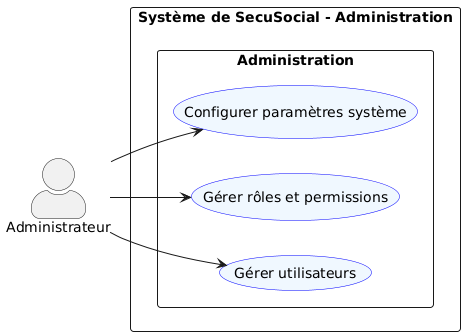
\includegraphics[width=0.5\textwidth]{AdminUC.png}
\caption{Diagramme de cas d'utilisation - Administrateur}
\end{figure}

\newpage

\noindent Le deuxième diagramme illustre les fonctionnalités accessibles aux contacts des entreprises clientes. Ils peuvent gérer les informations de \textbf{leur entreprise}, \textbf{leurs travailleurs} et \textbf{créer et suivre des demandes DIMONA}.

\vspace{0.5cm}
\begin{figure}[h]
\centering
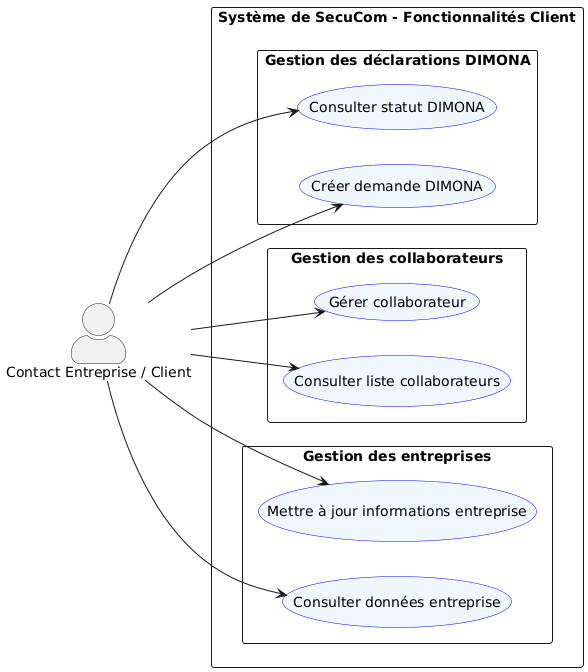
\includegraphics[width=0.5\textwidth]{ClientUC.png}
\caption{Diagramme de cas d'utilisation - Client}
\end{figure}

\noindent Le troisième diagramme présente les fonctionnalités accessibles aux employés du secrétariat social. Ils disposent d'un accès étendu pour \textbf{gérer les entreprises clientes}, \textbf{leurs travailleurs} et \textbf{traiter les demandes DIMONA ainsi que leurs statuts}. Le système intervient également pour certaines actions automatisées comme les notifications.

\vspace{0.5cm}
\begin{figure}[h]
\centering
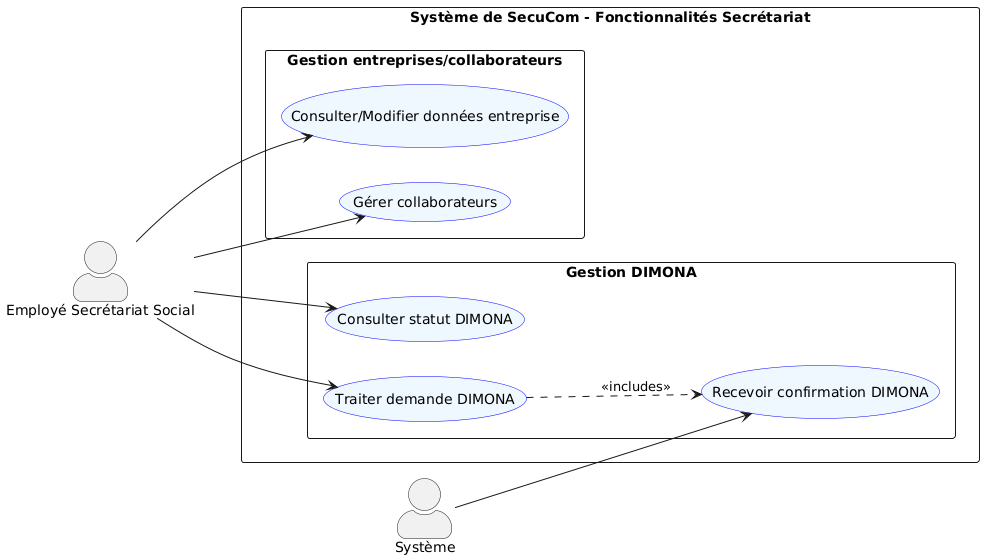
\includegraphics[width=0.5\textwidth]{SecretariatUC.png}
\caption{Diagramme de cas d'utilisation - Secrétariat Social}
\end{figure}

\section{Exigences et besoins techniques, de sécurité et de performance}

\subsection{Besoins techniques}

L'architecture technique de SecuCom doit répondre aux exigences spécifiques d'un secrétariat social tout en garantissant évolutivité, maintenabilité et robustesse. Les besoins techniques identifiés sont les suivants :

\vspace{0.5cm}
\textbf{Architecture globale} :
\begin{itemize}[leftmargin=*,label=\textcolor{darkgray}{$\bullet$},itemsep=0.3em]
  \item Architecture permettant une séparation claire entre l'interface utilisateur et la logique métier
  \item Communication efficace entre les différentes couches du système
  \item Flexibilité dans les options de déploiement selon les besoins
\end{itemize}


\vspace{0.5cm}
\textbf{Interface utilisateur} :
\begin{itemize}[leftmargin=*,label=\textcolor{darkgray}{$\bullet$},itemsep=0.3em]
  \item Interface intuitive et facile à prendre en main
  \item Adaptation à différentes tailles d'écran desktop (pas d'optimisation mobile requise)
  \item Gestion efficace des états et des données affichées
\end{itemize}


\vspace{0.5cm}
\textbf{Traitement des données} :
\begin{itemize}[leftmargin=*,label=\textcolor{darkgray}{$\bullet$},itemsep=0.3em]
  \item Système robuste de gestion de l'authentification et des autorisations
  \item Mécanismes efficaces pour l'accès et la persistance des données
  \item Solution adaptée pour le stockage sécurisé des données structurées
\end{itemize}


\vspace{0.5cm}
\textbf{Environnement de développement} :
\begin{itemize}[leftmargin=*,label=\textcolor{darkgray}{$\bullet$},itemsep=0.3em]
  \item Gestion de version pour le suivi des modifications
  \item Processus de build automatisé pour faciliter le développement
\end{itemize}

\subsection{Besoins de sécurité}

La sécurité est un aspect fondamental de SecuCom, étant donné la nature sensible des données traitées. Les exigences de sécurité suivantes ont été identifiées :


\vspace{0.5cm}
\textbf{Authentification et autorisation} :
\begin{itemize}[leftmargin=*,label=\textcolor{darkgray}{$\bullet$},itemsep=0.3em]
  \item Système d'authentification sécurisé avec gestion de jetons d'accès
  \item Gestion fine des rôles et permissions pour différents types d'utilisateurs
  \item Séparation stricte des espaces de données entre les différentes entreprises clientes
  \item Validation systématique des permissions à chaque requête
\end{itemize}


\newpage
\textbf{Protection des données} :
\begin{itemize}[leftmargin=*,label=\textcolor{darkgray}{$\bullet$},itemsep=0.3em]
  \item Transmission sécurisée des données via des protocoles chiffrés
  \item Gestion appropriée des exceptions pour éviter la fuite d'informations sensibles
  \item Conformité au RGPD (Règlement Général sur la Protection des Données)
\end{itemize}


\vspace{0.5cm}
\textbf{Sécurité applicative} :
\begin{itemize}[leftmargin=*,label=\textcolor{darkgray}{$\bullet$},itemsep=0.3em]
  \item Protection contre les attaques courantes (XSS, CSRF, injection SQL)
  \item Validation rigoureuse des entrées utilisateur
  \item Gestion sécurisée des mots de passe avec techniques de hachage appropriées
  \item Mécanisme de rafraîchissement des jetons d'authentification
\end{itemize}

\subsection{Besoins de performance}

Bien qu'aucune restriction spécifique n'ait été définie en termes de performance, SecuCom doit offrir une expérience utilisateur fluide et réactive pour garantir son adoption par les utilisateurs. Les exigences suivantes ont été établies :


\vspace{0.5cm}
\textbf{Temps de réponse} :
\begin{itemize}[leftmargin=*,label=\textcolor{darkgray}{$\bullet$},itemsep=0.3em]
  \item Chargement initial de l'application < 3 secondes
  \item Temps de réponse des requêtes < 1 seconde pour les opérations courantes
  \item Affichage des listes et tableaux optimisé
\end{itemize}


\vspace{0.5cm}
\textbf{Capacité et évolutivité} :
\begin{itemize}[leftmargin=*,label=\textcolor{darkgray}{$\bullet$},itemsep=0.3em]
  \item Capacité à gérer la croissance du nombre d'entreprises clientes et de collaborateurs
  \item Architecture permettant l'évolutivité en cas de besoin
\end{itemize}


\vspace{0.5cm}
\textbf{Optimisation} :
\begin{itemize}[leftmargin=*,label=\textcolor{darkgray}{$\bullet$},itemsep=0.3em]
  \item Requêtes optimisées pour les opérations courantes
\end{itemize}

\vspace{1cm}

\begin{tcolorbox}[
  title={\textbf{Cadre des exigences}},
  colback=blue!5!white,
  colframe=primarycolor,
  fonttitle=\bfseries,
  boxrule=0.5mm,
  arc=2mm,
  left=6mm,
  right=6mm,
  top=6mm,
  bottom=6mm
]
Ces exigences techniques, de sécurité et de performance constituent le cadre dans lequel SecuCom doit être développé, garantissant une solution robuste, sécurisée et performante qui répond aux besoins spécifiques de Sodabel et potentiellement d'autres secrétariats sociaux de taille similaire à l'avenir.
\end{tcolorbox}
